\documentclass{report}
\usepackage{listings}
\usepackage[margin=1.0in]{geometry}
\usepackage{graphicx}
\usepackage{hyperref}
\usepackage{amsmath}
\hypersetup{colorlinks=true}
\usepackage[document]{}
\title{EECE.5200 - Homework 5}
\author{Travis Kessler}
\date{30 March 2021}
\begin{document}
	\maketitle
	\newpage

	\lstset{frame=lines}

	\section*{Accessing Source Code}
	
	Source code is available at: \href{https://github.com/tjkessler/eece5200/tree/main/hw5}{https://github.com/tjkessler/eece5200/tree/main/hw5}
	
	\textit{}
	
	\noindent To run the code, first run \textbf{\textit{make}} in the \textit{hw5} directory. This will create one output file, \textbf{q1.o}. This executable will output all information relevant to the assignment, and export data to two files for plotting with \textbf{plot\_results.py}.

	\section*{Question 1}
	
	Given the function $e^z$, determine the $N + 1$ term Chebyshev expansion valid for $0 \leq z \leq 1$:
	
	\begin{center}
		
		$e^z = \sum_{n=0}^{N}a_n T_n (x)$

	\end{center}

	\noindent Assume a map between $z$ and $x$ is given algebraically as $x = 2z - 1 \implies z = (x + 1) / 2 \implies$
	
	\begin{center}
		$e^{(x+1) / 2} = \sum_{n=0}^{N}a_n T_n (x)$
	\end{center}

	\noindent where $-1 \leq x \leq 1$.
	
	\subsection*{a.}
	
	Given that $N = 8$, the coefficients $\underline{a} = [a_0, ..., a_N]$ are found by minimizing the residual at the extreme points of $T_N$, defined as $x_i = cos(\theta_i)$ where $\theta_i = i \pi / N$ for $i = (0, N)$. The system of variables can be re-written as:
	
	\begin{center}

		$\underline{f} = [T]\underline{a}$

	\end{center}

	\noindent where $\underline{f}$ is a vector of solutions for $e^{(x_i+1) / 2}$, $\underline{a}$ are unknown coefficients, and $[T]$ is a matrix representation of first-kind Chebyshev polynomials. Upon calling $gess$, the coefficients $\underline{a}$ were found to be:
	
	\begin{lstlisting}
 Coefficients a:
a           0  =    1.75338769    
a           1  =   0.850391567    
a           2  =   0.105208702    
a           3  =    8.72212369E-03
a           4  =    5.43408096E-04
a           5  =    2.71295994E-05
a           6  =    1.12497901E-06
a           7  =    3.78512972E-08
a           8  =   -1.62590919E-08
	\end{lstlisting}

	\noindent it is observed that the magnitudes of the first three coefficients are considerably larger than the remaining coefficients. This likely indicates that a lower-order Chebyshev polynomial system, perhaps $N = 3$, can be used to adequately represent the function $e^z$.
	
\subsection*{b.}

	The error between approximate and exact results calculated using $M$ uniformly distributed values of $z$ where $0 \leq z \leq 1$ and $i = (1, M)$ is determined using the mean absolute error, defined as:
	
	\begin{center}

	$MAE = \frac{\sum_{i=1}^{M} | y_i - \hat{y}_i |}{M}$

	\end{center}

	\noindent where $y_i$ is an exact solution for $e^{z_i}$ and $\hat{y}_i$ is an approximate solution given known coefficients $\underline{a}$. The approximate solution is computed using:
	
	\begin{center}
		
		$\hat{y}_i = \sum_{j=0}^{N}\underline{a}_j T_j $
		
	\end{center}

	\noindent where $T$ is a vector length $N$ with initial conditions $T_0 = 1.0$ and $T_1 = 2z_i - 1$. The remaining $j=(2, N)$ values are calculated with:
	
	\begin{center}
		
		$T_j = 2T_{j-1}(2z_i - 1) - T_{j-2}$
		
	\end{center}

	\noindent The following output was achieved when determining the error of the approximate solution with $M = 16$, and the parity between values is displayed in Figure 1:
	
	\begin{lstlisting}
Interval=16; actual e^z compared to Cheb. derived:
Actual Chebyshev-Derived
1.00000000       1.00000012    
1.06449449       1.06449461    
1.13314843       1.13314867    
1.20623028       1.20623052    
1.28402543       1.28402543    
1.36683798       1.36683798    
1.45499146       1.45499146    
1.54883027       1.54883039    
1.64872122       1.64872122    
1.75505471       1.75505459    
1.86824596       1.86824596    
1.98873746       1.98873734    
2.11700010       2.11699986    
2.25353479       2.25353503    
2.39887524       2.39887547    
2.55358934       2.55358958    
2.71828175       2.71828175    
Given 16 samples of z, mean absolute error =    2.02655792E-06
	\end{lstlisting}
	
	\begin{figure}[!ht]
		\centering
		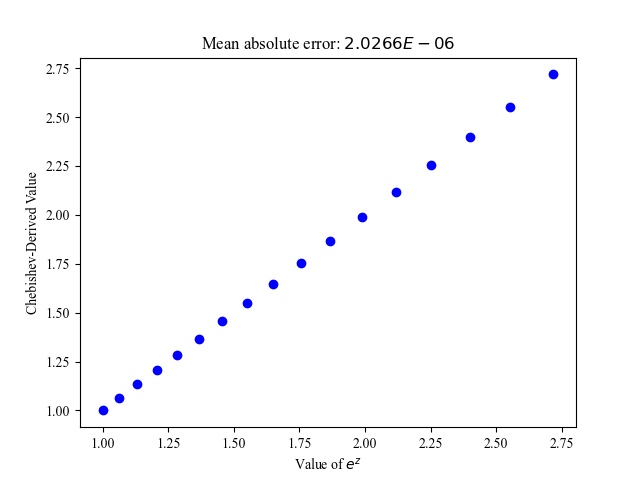
\includegraphics[scale=0.7]{figures/results_partb.png}
		\caption{Parity between approximate results and exact results}
	\end{figure}

\subsection*{c.}

	In a discrete system, we define the derivative as the forward difference operator, $\Delta$, applied to two consecutive points in a uniformly distributed series of length $N$:
	
	\begin{center}
		
		$\Delta f = n \rightarrow f_{i + 1} - f_i$
		
	\end{center}

	\noindent In this application, the difference operator is applied to both exact and approximate data from subsection (b). Upon executing the previously mentioned error calculation procedure, the following output was achieved when determining the error of the approximate solution's derivative, and the parity between exact and approximate derivatives is displayed in Figure 2:
	
	\begin{lstlisting}
dz=16; deriv. of actual compared to Cheb. derived:
Actual Chebyshev-Derived
6.44944906E-02   6.44944906E-02
6.86539412E-02   6.86540604E-02
7.30818510E-02   7.30818510E-02
7.77951479E-02   7.77949095E-02
8.28125477E-02   8.28125477E-02
8.81534815E-02   8.81534815E-02
9.38388109E-02   9.38389301E-02
9.98909473E-02   9.98908281E-02
0.106333494      0.106333375    
0.113191247      0.113191366    
0.120491505      0.120491385    
0.128262639      0.128262520    
0.136534691      0.136535168    
0.145340443      0.145340443    
0.154714108      0.154714108    
0.164692402      0.164692163    
Deriv. mean absolute error:    1.11758709E-07
	\end{lstlisting}

	\begin{figure}[!ht]
		\centering
		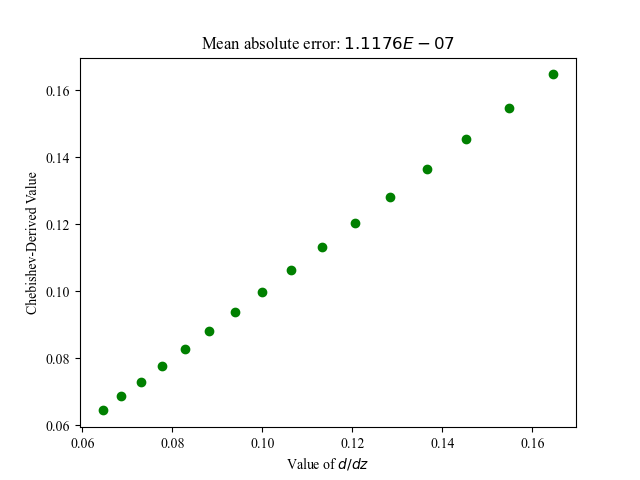
\includegraphics[scale=0.7]{figures/results_partc.png}
		\caption{Parity between approximate derivative and exact derivative}
	\end{figure}

\newpage

	\begin{thebibliography}{99\kern\bibindent}
	
	\bibitem{hwref}
	Thompson, C.
	\textit{University of Massachusetts Lowell Department of Electrical and Computer Engineering 16.520 Computer Aided Engineering Analysis Problem Set 6}.
	Retrieved March 30, 2021, from http://morse.uml.edu/Activities.d/16.520/S2021.d/HW5.pdf
	
	\end{thebibliography}

\end{document}